%-*- coding: UTF-8 -*-
% gougu.tex
% 勾股定理
% 使用 xelatex 编译文档时,ctexart 文档类会调用 xeCJK 宏包
% \documentclass[UTF8]{article} 这个就不会在页眉显示目录的内容
%\documentclass[UTF8]{ctexart} % 这个就时在页眉显示目录内容的原因
\documentclass[fontset=windows, 12pt]{article}
\usepackage{ctex} % ctexart会默认调用相关的中文包
\usepackage{graphicx}
\usepackage{float}
\usepackage{geometry}
\usepackage[format=hang,font=small,textfont=it]{caption}
\usepackage[nottoc]{tocbibind}
% 添加参考文献目录


% 另外一种添加目录的方法E
% \addcontentsline{nottoc}{section}{参考文献}
\title{杂谈勾股定理}
\author{Eurake}
\date{\today}
\bibliographystyle{plain}
\geometry{a4paper,centering,scale=0.8}
% 声明了参考文献的格式
% \cite 命令的参数 Kline 和 quanjing 分别是其中两篇的引用标签, 也就是在 math.bib
% 中每个条目第一行出现的东西。
% 如果要在列表中显示并不直接引用的文献,可以使用 \nocite 命令

% 编译步骤如下
% xelatex [处理对象:gougu.tex]:运行xelatex为bibtex准备好辅助文件,确定数据库中的哪些文献将被列出来\emph{}
% bibtex  [处理对象:gougu.aux]:bibtex 处理辅助文件 gougu.aux,从文献数据库中选取文献,按指定的格式【plain】生成文献列表的 LATEX 代码。
% xelatex [处理对象:gougu.tex]:把引用的文献添加到文章中【末尾】
% xelatex [处理对象:gougu.tex]:使用 \cite 命令会在引用的位置显示文献在列表中的编号
% 第三四次:后面两次 xelatex 再读入文献列表代码并生成正确的引用信息。

\newtheorem{thm}{定理}

\newenvironment{myquote}
	{\begin{quote}
		\kaishu
		\zihao{-5}
	}
	{\end{quote}}

\newcommand\degree{^\circ}
\newcommand{\Test}{This is A Test For Macro In TexStudio}
% 可以使用Ctrl + <-【->】在不同的占位符之间跳转
\newcommand{\test}[1][default]{#1}
% 导言区定义环境的用法:
% 1. \newtheorem{name of theorem environment}{theorem environment label}
% 2. 导言区的{thm}{theorem label}说明以后的thm定理环境里的定理都被命名为定理1,定理2,……的格式
% 3.调用格式
% \begin{name of theorem environment}[the name of a theorem]
% 具体的定理内容
% \end{name of theorem environment}
% \newenvironment{myquote}
% {\begin{quote}\kaishu\zihao{-5}}
% {\end{quote}}




\begin{document}
\maketitle
\tableofcontents
\newpage

\begin{abstract}
	这是一篇关于勾股定理的背景与实际应用的文章。
\end{abstract}

\vspace*{4em}
\section{勾股定理在古代}
西方称勾股定理为毕达哥拉斯定理,将勾股定理的发现归功于公元前6世纪的毕达哥拉斯学派\cite{Kline}。该学派得到了一个法则,可以求出可排成直角三角形三边的三元数组。毕达哥拉斯学派没有书面著作,该定理的严格表述和证明则见于欧几里德\footnote{欧几里德,约公元前330--275 年}
《几何原本》的命题47:“直角三角形斜边上的正方形等于两直角边上的个正方形之和。”证明是用面积做的。我国《周髀算经》载商高(约公元前12世纪)答周公问:

\begin{myquote}
	勾广三,股修四,径隅五。
\end{myquote}

又载陈子(约公元前 7--6 世纪)答荣方问:

\begin{quote}
	\zihao{-5}\kaishu
	若求邪至日者,以日下为勾,日高为股,勾股各自乘,并而开方除	 之,得邪至日。
\end{quote}

都较古希腊更早。后者已经明确道出勾股定理的一般形式。图 \ref{fig:xiantu} 是我国古代对勾股定理的一种证明 \cite{quanjing}。

% 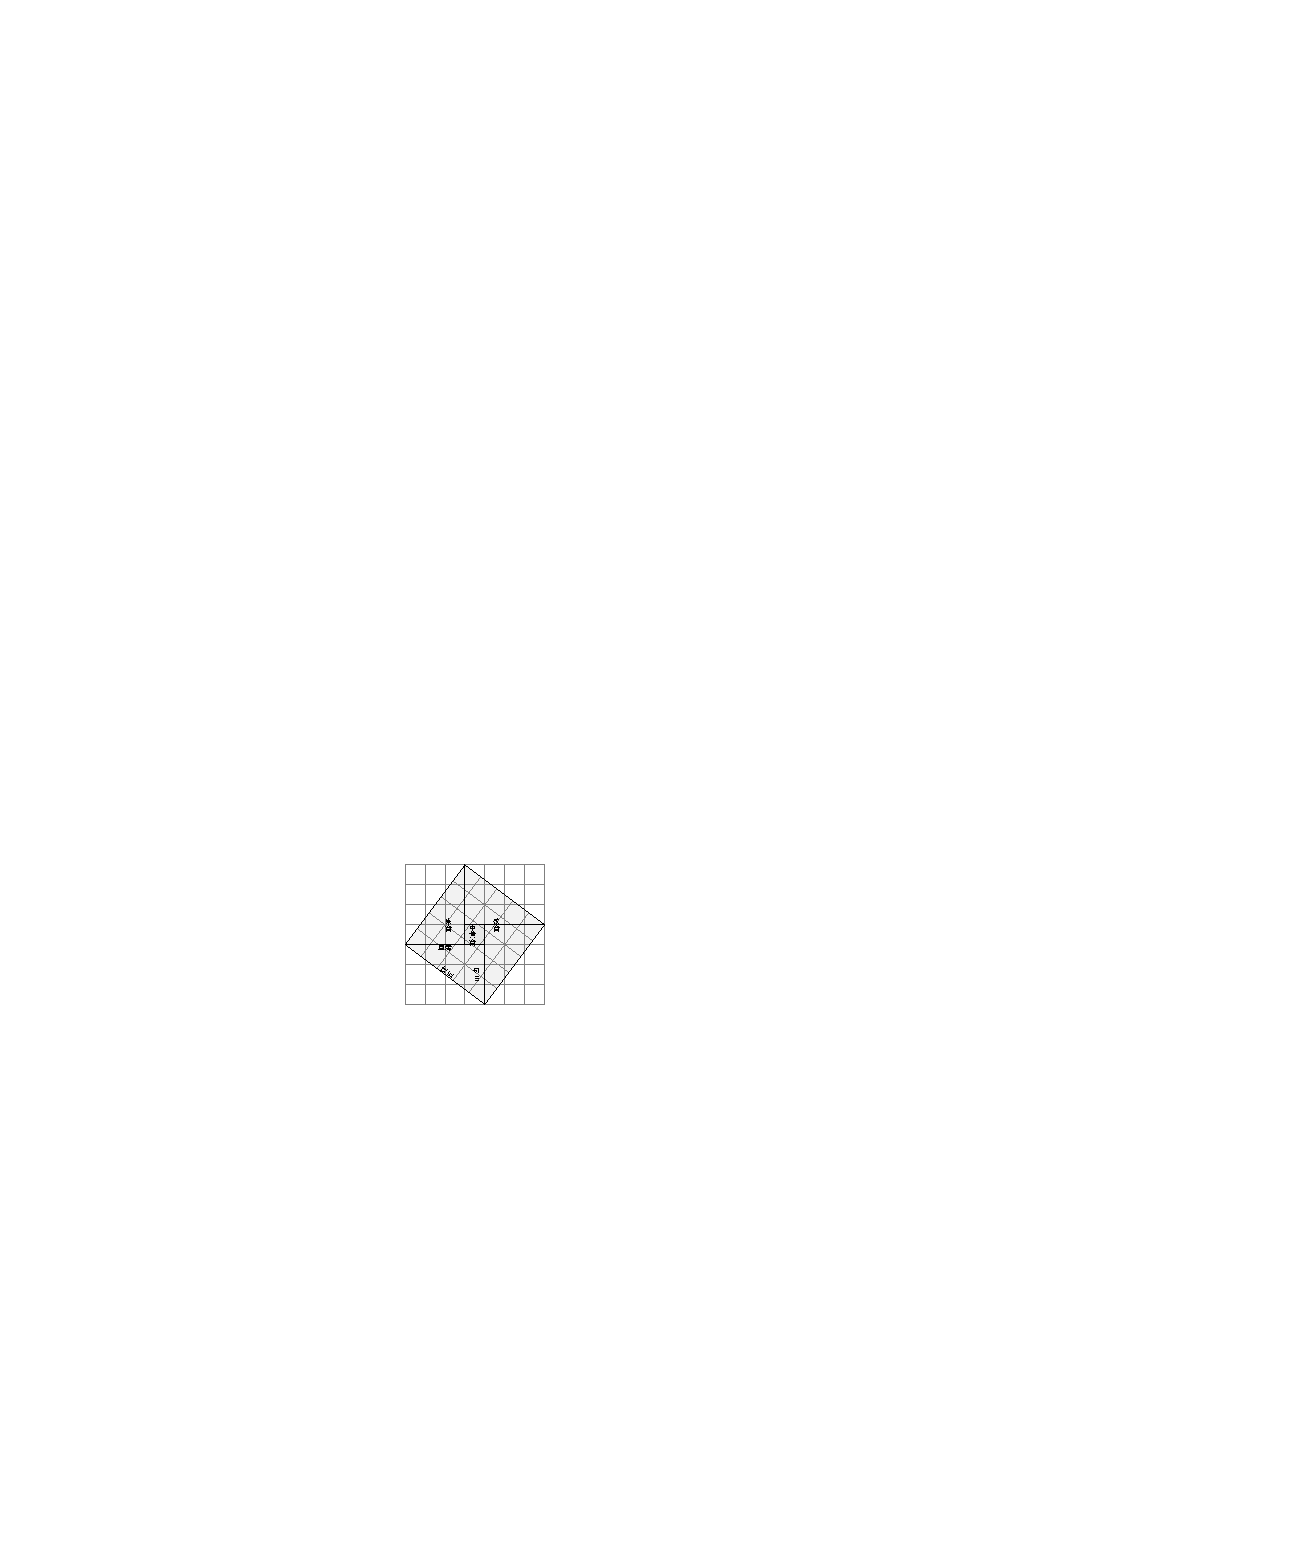
\includegraphics[width=3cm]{xiantu.pdf}
% 这种引入图片会造成图片文字混杂,因为latex把图片的文字同等看待了

\begin{figure}[ht]
	\centering
	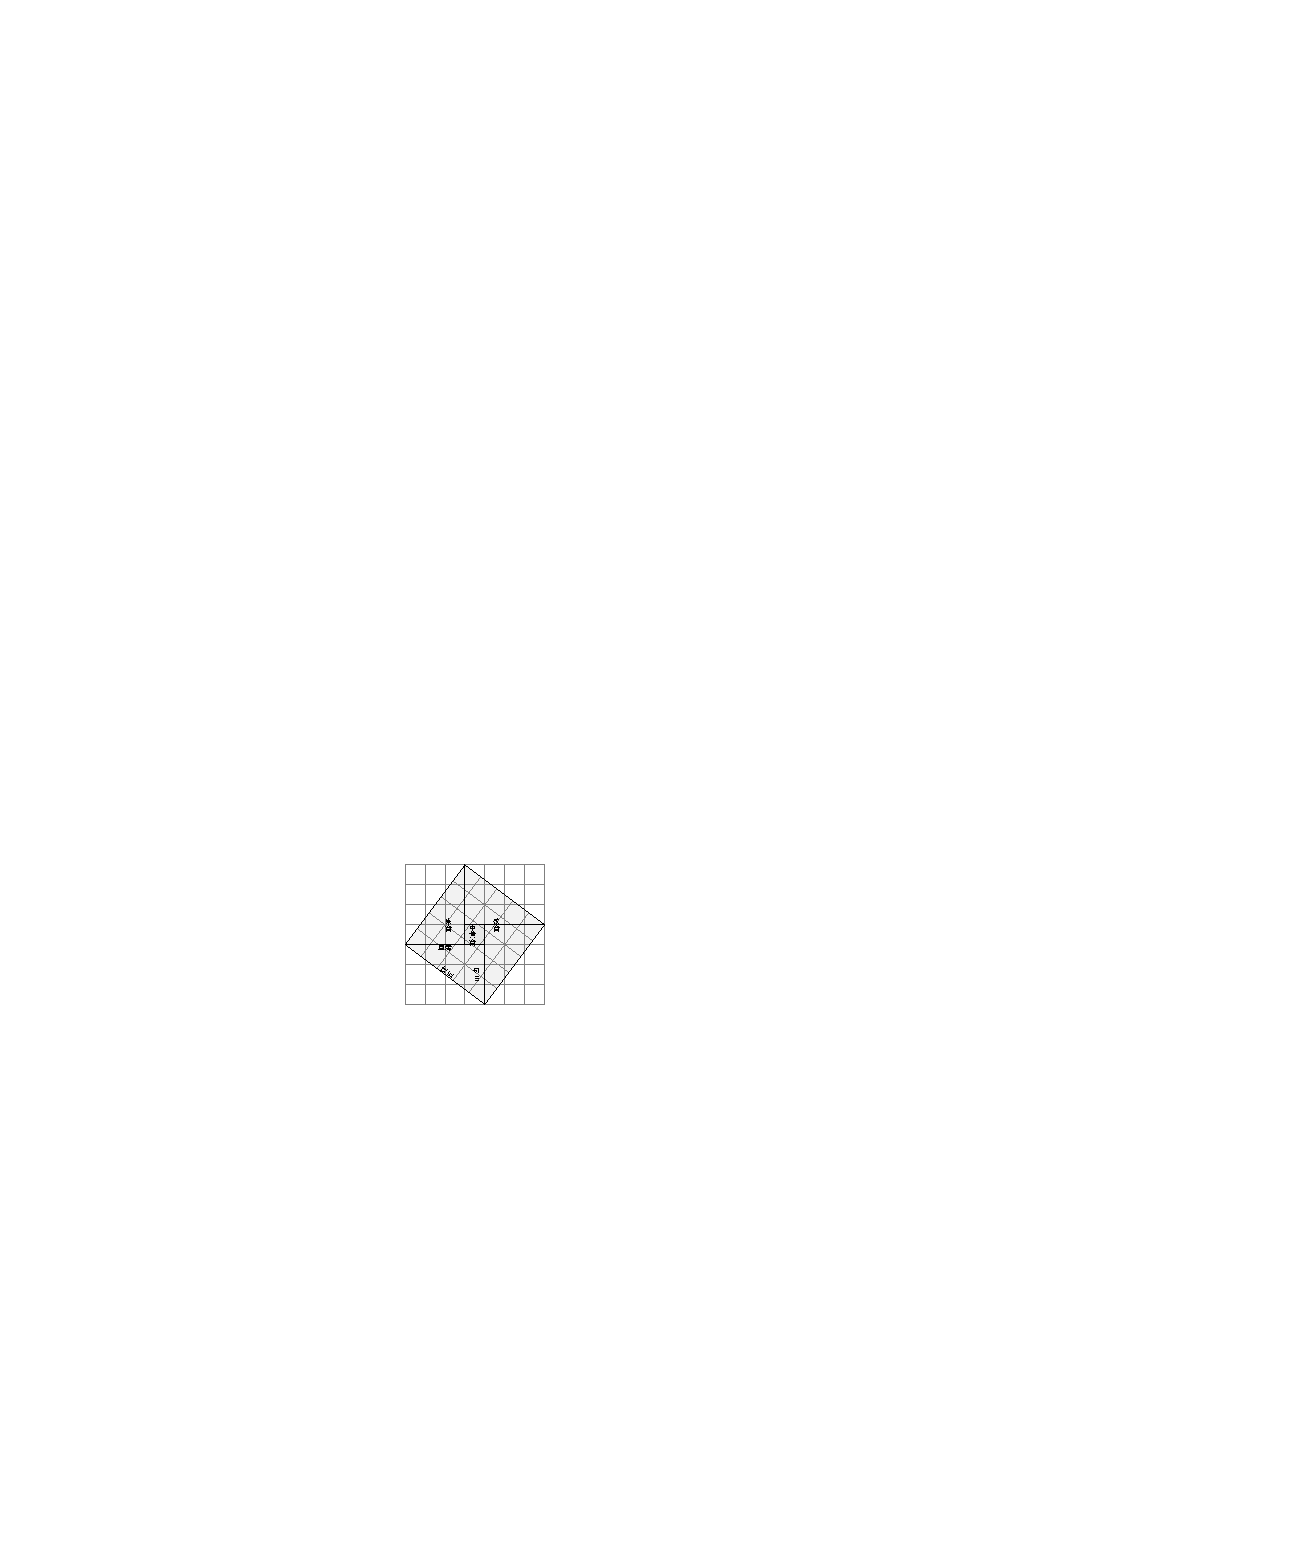
\includegraphics[scale=2]{xiantu.pdf}
	\caption{宋赵爽在《周髀算经》注中作的弦图(仿制),该图给出了勾股定
	理的一个极具对称美的证明。}
	\label{fig:xiantu}
\end{figure}

\section{勾股定理的近代形式}
勾股定理可以用现代语言表述如下:

\begin{thm}[勾股定理]
	直角三角形斜边的平方等于两腰的平方和。

	可以用符号语言表述为:设直角三角形ABC,其中
	$ \angle C = 90\degree $,则有
	\begin{equation}
		AB^2 = BC^2 + AC^2
	\end{equation}
\end{thm}
满足式 (1) 的整数称为勾股数。第 1 节所说毕
达哥拉斯学派得到的三元数组就是勾股数。下表列
出一些较小的勾股数:
\begin{table}[H]
	\begin{tabular}{|r|r|r|}
		\hline
		直角边 $a$ & 直角边 $b$ & 斜边 $c$ \\
		\hline
		3 & 4  & 5 \\
		5 & 12 & 13 \\
		\hline
	\end{tabular}	%	
	\qquad
	$a^2 + b^2 = c^2$
\end{table}
\nocite{Shiye}
% 显示未被直接引用的文献
\bibliography{math}
% 用 \bibliography 命令要求打印出参考文献列表E
\end{document}

LaTeX总结:
  LATEX 是一种结构化的排版语言,在填写标准格式的模板时(就像我们填写 1.2.2 节
所列的提纲一样)可以忽略编号、格式等许多具体细节。在文档排版中应该主动
追求内容与格式的分离,在 document 环境之内避免直接使用诸如字体字号、对齐缩进
的格式控制命令,而代之以有具体意义的环境和命令,让文档变得清晰。这种模式化的
操作能提高工作效率,许多 LATEX 的拥护者把这种工作方式称为“所想即所得x”。可是
不要忘记,机器还远没有智能化到想人之所想的程度,LATEX 也不能阻止我们编排出效
果糟糕、代码混乱的文章,要得到好的文章,无论是在内容上还是排版形式上,都得靠
我们自己。










